% Options for packages loaded elsewhere
\PassOptionsToPackage{unicode}{hyperref}
\PassOptionsToPackage{hyphens}{url}
%
\documentclass[
  12pt,
  a4paper,
  DIV=11,
  numbers=noendperiod]{scrreprt}

\usepackage{amsmath,amssymb}
\usepackage{setspace}
\usepackage{iftex}
\ifPDFTeX
  \usepackage[T1]{fontenc}
  \usepackage[utf8]{inputenc}
  \usepackage{textcomp} % provide euro and other symbols
\else % if luatex or xetex
  \usepackage{unicode-math}
  \defaultfontfeatures{Scale=MatchLowercase}
  \defaultfontfeatures[\rmfamily]{Ligatures=TeX,Scale=1}
\fi
\usepackage{lmodern}
\ifPDFTeX\else  
    % xetex/luatex font selection
\fi
% Use upquote if available, for straight quotes in verbatim environments
\IfFileExists{upquote.sty}{\usepackage{upquote}}{}
\IfFileExists{microtype.sty}{% use microtype if available
  \usepackage[]{microtype}
  \UseMicrotypeSet[protrusion]{basicmath} % disable protrusion for tt fonts
}{}
\usepackage{xcolor}
\setlength{\emergencystretch}{3em} % prevent overfull lines
\setcounter{secnumdepth}{5}
% Make \paragraph and \subparagraph free-standing
\ifx\paragraph\undefined\else
  \let\oldparagraph\paragraph
  \renewcommand{\paragraph}[1]{\oldparagraph{#1}\mbox{}}
\fi
\ifx\subparagraph\undefined\else
  \let\oldsubparagraph\subparagraph
  \renewcommand{\subparagraph}[1]{\oldsubparagraph{#1}\mbox{}}
\fi


\providecommand{\tightlist}{%
  \setlength{\itemsep}{0pt}\setlength{\parskip}{0pt}}\usepackage{longtable,booktabs,array}
\usepackage{calc} % for calculating minipage widths
% Correct order of tables after \paragraph or \subparagraph
\usepackage{etoolbox}
\makeatletter
\patchcmd\longtable{\par}{\if@noskipsec\mbox{}\fi\par}{}{}
\makeatother
% Allow footnotes in longtable head/foot
\IfFileExists{footnotehyper.sty}{\usepackage{footnotehyper}}{\usepackage{footnote}}
\makesavenoteenv{longtable}
\usepackage{graphicx}
\makeatletter
\def\maxwidth{\ifdim\Gin@nat@width>\linewidth\linewidth\else\Gin@nat@width\fi}
\def\maxheight{\ifdim\Gin@nat@height>\textheight\textheight\else\Gin@nat@height\fi}
\makeatother
% Scale images if necessary, so that they will not overflow the page
% margins by default, and it is still possible to overwrite the defaults
% using explicit options in \includegraphics[width, height, ...]{}
\setkeys{Gin}{width=\maxwidth,height=\maxheight,keepaspectratio}
% Set default figure placement to htbp
\makeatletter
\def\fps@figure{htbp}
\makeatother

\KOMAoption{captions}{tableheading}
\usepackage{indentfirst}
\usepackage{float}
\floatplacement{figure}{H}
\usepackage{libertine}
\makeatletter
\@ifpackageloaded{caption}{}{\usepackage{caption}}
\AtBeginDocument{%
\ifdefined\contentsname
  \renewcommand*\contentsname{Содержание}
\else
  \newcommand\contentsname{Содержание}
\fi
\ifdefined\listfigurename
  \renewcommand*\listfigurename{Список иллюстраций}
\else
  \newcommand\listfigurename{Список иллюстраций}
\fi
\ifdefined\listtablename
  \renewcommand*\listtablename{Список таблиц}
\else
  \newcommand\listtablename{Список таблиц}
\fi
\ifdefined\figurename
  \renewcommand*\figurename{Рисунок}
\else
  \newcommand\figurename{Рисунок}
\fi
\ifdefined\tablename
  \renewcommand*\tablename{Таблица}
\else
  \newcommand\tablename{Таблица}
\fi
}
\@ifpackageloaded{float}{}{\usepackage{float}}
\floatstyle{ruled}
\@ifundefined{c@chapter}{\newfloat{codelisting}{h}{lop}}{\newfloat{codelisting}{h}{lop}[chapter]}
\floatname{codelisting}{Список}
\newcommand*\listoflistings{\listof{codelisting}{Листинги}}
\makeatother
\makeatletter
\makeatother
\makeatletter
\@ifpackageloaded{caption}{}{\usepackage{caption}}
\@ifpackageloaded{subcaption}{}{\usepackage{subcaption}}
\makeatother
\ifLuaTeX
\usepackage[bidi=basic]{babel}
\else
\usepackage[bidi=default]{babel}
\fi
\babelprovide[main,import]{russian}
\babelprovide[import]{english}
% get rid of language-specific shorthands (see #6817):
\let\LanguageShortHands\languageshorthands
\def\languageshorthands#1{}
\ifLuaTeX
  \usepackage{selnolig}  % disable illegal ligatures
\fi
\usepackage[backend=biber,langhook=extras,autolang=other*]{biblatex}
\addbibresource{bib/cite.bib}
\usepackage{csquotes}
\usepackage{bookmark}

\IfFileExists{xurl.sty}{\usepackage{xurl}}{} % add URL line breaks if available
\urlstyle{same} % disable monospaced font for URLs
\hypersetup{
  pdftitle={Шаблон отчёта по лабораторной работе},
  pdfauthor={Дмитрий Сергеевич Кулябов},
  pdflang={ru-RU},
  hidelinks,
  pdfcreator={LaTeX via pandoc}}

\title{Шаблон отчёта по лабораторной работе}
\usepackage{etoolbox}
\makeatletter
\providecommand{\subtitle}[1]{% add subtitle to \maketitle
  \apptocmd{\@title}{\par {\large #1 \par}}{}{}
}
\makeatother
\subtitle{Простейший вариант}
\author{Дмитрий Сергеевич Кулябов}
\date{}

\begin{document}
\maketitle

\renewcommand*\contentsname{Содержание}
{
\setcounter{tocdepth}{1}
\tableofcontents
}
\listoffigures
\listoftables
\setstretch{1.5}
\chapter{Цель
работы}\label{ux446ux435ux43bux44c-ux440ux430ux431ux43eux442ux44b}

Здесь приводится формулировка цели лабораторной работы. Формулировки
цели для каждой лабораторной работы приведены в методических указаниях.

Цель данного шаблона --- максимально упростить подготовку отчётов по
лабораторным работам. Модифицируя данный шаблон, студенты смогут без
труда подготовить отчёт по лабораторным работам, а также познакомиться с
основными возможностями разметки Markdown.

\chapter{Задание}\label{ux437ux430ux434ux430ux43dux438ux435}

Здесь приводится описание задания в соответствии с рекомендациями
методического пособия и выданным вариантом.

\chapter{Теоретическое
введение}\label{ux442ux435ux43eux440ux435ux442ux438ux447ux435ux441ux43aux43eux435-ux432ux432ux435ux434ux435ux43dux438ux435}

Здесь описываются теоретические аспекты, связанные с выполнением работы.

Например, в табл.~\ref{tbl-std-dir} приведено краткое описание
стандартных каталогов Unix.

\begin{longtable}[]{@{}
  >{\raggedright\arraybackslash}p{(\columnwidth - 2\tabcolsep) * \real{0.1014}}
  >{\raggedright\arraybackslash}p{(\columnwidth - 2\tabcolsep) * \real{0.8986}}@{}}
\caption{Описание некоторых каталогов файловой системы GNU
Linux}\label{tbl-std-dir}\tabularnewline
\toprule\noalign{}
\begin{minipage}[b]{\linewidth}\raggedright
Имя каталога
\end{minipage} & \begin{minipage}[b]{\linewidth}\raggedright
Описание каталога
\end{minipage} \\
\midrule\noalign{}
\endfirsthead
\toprule\noalign{}
\begin{minipage}[b]{\linewidth}\raggedright
Имя каталога
\end{minipage} & \begin{minipage}[b]{\linewidth}\raggedright
Описание каталога
\end{minipage} \\
\midrule\noalign{}
\endhead
\bottomrule\noalign{}
\endlastfoot
\texttt{/} & Корневая директория, содержащая всю файловую \\
\texttt{/bin} & Основные системные утилиты, необходимые как в
однопользовательском режиме, так и при обычной работе всем
пользователям \\
\texttt{/etc} & Общесистемные конфигурационные файлы и файлы
конфигурации установленных программ \\
\texttt{/home} & Содержит домашние директории пользователей, которые, в
свою очередь, содержат персональные настройки и данные пользователя \\
\texttt{/media} & Точки монтирования для сменных носителей \\
\texttt{/root} & Домашняя директория пользователя \texttt{root} \\
\texttt{/tmp} & Временные файлы \\
\texttt{/usr} & Вторичная иерархия для данных пользователя \\
\end{longtable}

Более подробно про Unix см. в
\autocite{tanenbaum_book_modern-os_ru,robbins_book_bash_en,zarrelli_book_mastering-bash_en,newham_book_learning-bash_en}.

\chapter{Выполнение лабораторной
работы}\label{ux432ux44bux43fux43eux43bux43dux435ux43dux438ux435-ux43bux430ux431ux43eux440ux430ux442ux43eux440ux43dux43eux439-ux440ux430ux431ux43eux442ux44b}

Описываются проведённые действия, в качестве иллюстрации даётся ссылка
на иллюстрацию (рис.~\ref{fig-001}).

\begin{figure}

\centering{

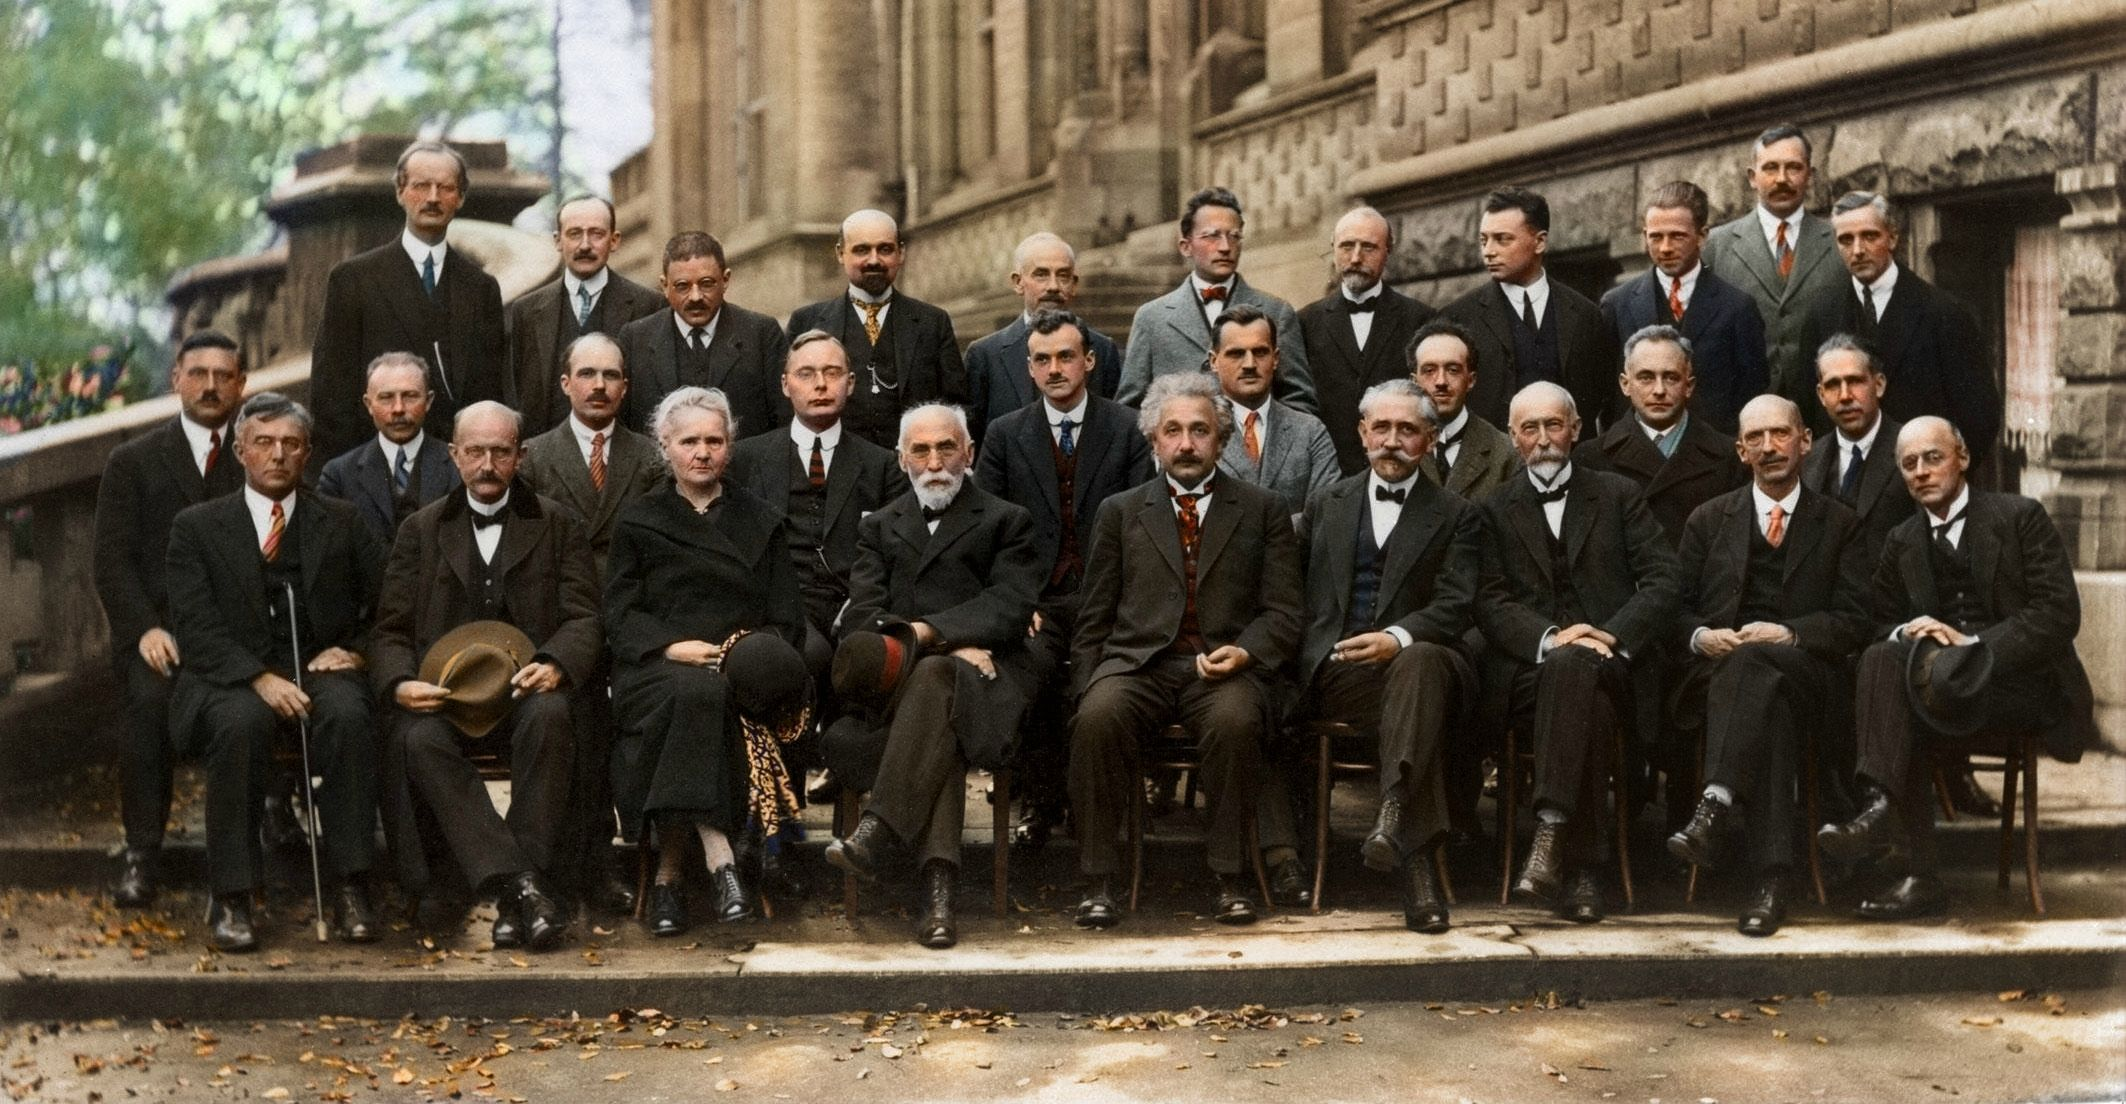
\includegraphics[width=0.7\textwidth,height=\textheight]{image/solvay.jpg}

}

\caption{\label{fig-001}V Сольвеевский конгресс (1927) «Электроны и
фотоны»}

\end{figure}%

\chapter{Выводы}\label{ux432ux44bux432ux43eux434ux44b}

Здесь кратко описываются итоги проделанной работы.

\chapter*{Список
литературы}\label{ux441ux43fux438ux441ux43eux43a-ux43bux438ux442ux435ux440ux430ux442ux443ux440ux44b}
\addcontentsline{toc}{chapter}{Список литературы}

\printbibliography[heading=none]




\end{document}
